\section{Project Dynamics}

Before commencing work upon the project, the team has discussed and finalised how they intend to operate as a unit which includes a software methodology to follow, a set of common software tools and meeting dynamics.

\subsection{Team Member Strengths}
\label{sec:TeamStrengths}
The strengths of each team member have been identified and are summarised in the following table:

\begin{table}[ht]
\centering
\begin{tabular}{l | l}
Team & Strengths \\\hline
Michael Harris & Coding, LaTeX and leading \\
Jonathan Harrison & Note taking, organisation, time keeping, web design and coding  \\
Samantha Kanza & LaTeX, organisation, web design and coding  \\
Jennifer Lantair & Coding, LaTeX, proof reading and organisation  \\
\end{tabular}
\caption{Team Member Strengths}
\end{table}
\label{tab:TeamStrengths} 

\subsection{Job Roles}
Using each team member's strengths as described in Section \ref{sec:TeamStrengths}, as well as knowledge from previous experiences together, the team members have been assigned the following roles. These roles are not all inclusive, that is to say that no role is intended to describe all of a team member's work. The roles are laid out in the following table:

\begin{table}[ht]
\centering
\begin{tabular}{l | l}
Team & Roles\\\hline
Michael Harris & Project Manager \\
Jonathan Harrison & Secretary and Time Manager \\
Samantha Kanza & System Architect  \\
Jennifer Lantair & Documenter  \\
\end{tabular}
\caption{Team Roles}
\end{table}
\label{tab:TeamRoles} 

In addition to these roles each team member shall also be working upon the tasks involved with each stage of the project such as the system implementation and documentation. Each team member is intended to be working for approximately equal time periods over the ten weeks of the project to ensure fair division of the work load.

\subsection{Software Model}
\label{sec:SoftwareModel}
The project will be completed in a relatively short time scale (only ten weeks) therefore it calls for a rapid iterative software engineering process to ensure that no time is wasted. Therefore we have decided to go with the Iterative Waterfall model; the basic processes and the way the feedback works is shown in the following figure:

\begin{figure}[h1]
\begin{center}
 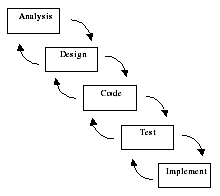
\includegraphics[trim = 0mm 0mm 0mm 0mm, clip, scale=0.6]{Images/iterativewaterfallmodel.png}
  \caption{The Iterative Waterfall model}\label{fig:iterativeWaterfall}
 \end{center}
\end{figure}

The Iterative Waterfall model, which is a variation of the original waterfall model, takes into account the work of Winston 
Royce \cite{Royce} who advocated the use of feedback in the waterfall model. The Iterative Waterfall model allows 
feedback to be generated in such an area as design and to step back a stage to the requirements if necessary. The ability to repeat a stage was believed by Royce to produce superior products. Royce was also a great believer in the power of strong contacts with a team's client. 
Such strong ties with the client meets the teams needs well because the production of a superior product which satisfies the client's requirements is desired. 

\subsection{Project Tools}
\label{sec:ProjectTools}
\label{sec:Tools}

The tools that the team have chosen to use throughout the project are detailed in the following Section. Tools chosen must be platform independent due to the different environments that each team member uses and they are familiar with them so that work can begin immediately with no additional learning curve.

\subsubsection{Communication Aids}
\label{sec:communicationAids}

The ability for the team to communicate effectively is very important, therefore the following tools were chosen in order that members could be contacted at all times:

\begin{itemize}
	\item{Email}
	\item{Google Chat/Talk}
	\item{Mobile Phones}
\end{itemize}

\subsubsection{Project Management}
\label{sec:ProjectManagement}

Project management tools are used as a means to manage elements of the project such as task and time management as well as ensuring all team members know when and where meetings and group work sessions shall occur. The following project management tools were selected:

\begin{itemize}
	\item{Google Calendar}
	\item{Microsoft Project}
\end{itemize}

\subsubsection{Documentation}

Documentation tools are those used to produce documentation during the project. The following documentation tools were used:

\begin{itemize}
	\item{Google Documents}
	\item{LaTeX Editors}
	\begin{itemize}
		\item{Kile}
		\item{TexWorks}
		\item{BibDesk}
	\end{itemize}
\end{itemize}

\subsubsection{Implementation}

The implementation tools which shall be used are as follows:
	
\begin{itemize}
	\item{Maven}
	\item{Eclipse with the following plugins:}
	\begin{itemize}
		\item{M2Eclipse (Maven plugin)}
		\item{SVN Team Provider (SVN plugin)}
	\end{itemize}
\end{itemize}

\subsubsection{Version Management}

A number of version management tools were considered for managing the teams documentation and coding bases. Those chosen were the following tools:

\begin{itemize}
	\item{UGForge}
	\item{Google Documents}
\end{itemize}

\subsection{Meetings}

The team has organised their internal and external meetings in the following sections. By organising these meetings the team hopes to ensure a structured environment for their project.

\subsubsection{Client/Supervisor Meeting}
The team intents to meet their supervisor and client at least once a week. These regular meetings will last a maximum of an hour and allow the team to discuss and evaluate current progress and tasks (which includes any problems that the team are having) and to plan and approve future work that will be done for next meeting.

The evaluation of progress and work during these regular meetings means that the team will get immediate feedback on their work ensuring that work meets the customer's expectations and requirements. These meetings lend themselves to the chosen software model detailed in Section \ref{sec:SoftwareModel}.

\subsubsection{Team Meetings}
\label{sec:TeamMeetings}
Beside Client/Supervisor meetings, the team shall have regular private meetings to allow the team to judge their current progress against their predicted progress as decided upon during the initial week of their project (see Appendix \ref{sec:GanttChart}). By doing this it will gauge whether the team are on track for their deadlines or if they are behind. In case of slippage the team may at these meetings call into effect their contingency plans which will place them back on schedule. 

These meetings shall last a maximum of an hour and will take place at the start and end of each week. Meetings at the beginning of the week shall occur on Mondays and will contain discussions about what the team has done over the weekend, plan the weeks goals and how they are to be divided and completed.

Finally, end of week meetings shall be every Friday and will follow Client/Supervisor meetings to allow for further discussion of points made in the previous meeting as well as plan work to be done over the weekend.

\subsection{Work Techniques}
The techniques that team members will be using whilst working on tasks throughout this project are detailed below.

\subsubsection{Logbooks}
Logbooks will be used by each team member to keep a record of their involvement with all areas of this project. Firstly, 
logbooks shall be used to plan activities, for example drawing out user interface designs and planning the implementation of modules.

As well as planning, while undertaking tasks the logbooks will be used to detail
the activity being done, the team members involved with that activity and the
number of minutes spent upon it. This is in order to help with keeping track of
the project's progress and to accurately update the project’s Gantt chart.

Finally logbooks should also be used as a private record of an individual's thoughts throughout the project in order that they can 
be used as reference when team members write their individual reports about the project.

\subsubsection{Peer Review}
\label{PeerReview}
Throughout the project, the team will peer review any completed tasks whereby team members besides those who completed the task will 
review the completed work in great detail in areas such as content and how it is written. Therefore any errors or inconsistencies will be easily spotted and can be corrected. Having these reviews ensures that work is completed to the same standard and is of the highest possible quality.

\subsubsection{Pair Programming}
\label{PairProgramming}
During the implementation of the project where appropriate the team will use the pair programming technique, where on one workstation one 
team member enters the code and the other team member overlooks the activity. Using this technique has a number of advantages:

\begin{itemize}
	\item{It's shown to reduce the number of man hours required to complete a project and it's size \cite{citePairProgramming}.}
	\item{It significantly decreases the likeliness of procrastination and the amount of time wasted on procrastination \cite{citeIlluminatedPair}.}
	\item{For a project where no individual team member has had prior experience in the subjects associated with this project e.g. video and audio processing. It provides benefits where the solution to a problem is unknown to the developers; two heads are better than one.}
	\item{Two team members will have an in depth understanding of any area of code.}
\end{itemize}

\subsection{Project Management}
The tools that the team members will be using to manage the project have already been stated in Section \ref{sec:Tools}, how we are going to use them are detailed below.

\subsubsection{Project and Task Management}
To successfully manage the project and to keep track of the progress of the project as a whole, a Gantt chart was produced using Microsoft Project 2010 and can be viewed in Appendix \ref{sec:GanttChart}. The Gantt chart contains:
\begin{itemize}
	\item{The project stages as per our Software Model (see section \ref{sec:SoftwareModel}).}
	\item{All the key tasks that are a part of this project.}
	\item{Milestones which include:}
	\begin{itemize}
		\item{Project deadlines such as Progress Seminars and Report Deliverables.}
		\item{Project stage milestones such as when the Implementation will be completed.}
		\item{Client/supervisor meetings.}
		\item{Contingency time to allow for the risks identified in Section \ref{sec:Risks} to be overcome.}
	\end{itemize}
\end{itemize}

This was updated on a weekly basis throughout the project prior to client/supervisor meetings held at the end of the week.

Using this chart, it allowed the team to evaluate their progress each week to ensure that all tasks were progressing at 
a reasonable rate and none were forgotten about. Furthermore, it has been used to evaluate our project which is detailed 
in Section \ref{sec:timeManagementEval}.

\subsubsection{Organisation}
In order to make sure that all team members had the same understanding of:
\begin{itemize}
	\item{When the project milestones occurred, as detailed in the Gantt chart.}
	\item{When and where any meetings were taking place.}
	\item{Other module deadlines/clashes that team members had.}
\end{itemize}

We decided to use Google Calendar due to the familiarity everyone had with using this software, it allowed everyone to be kept in sync and also, it could be viewed anywhere and at anytime across varying platforms and devices.

\subsection{Programming Styles}
\label{sec:ProgrammingStyles}
There are a large number of different coding practises and styles which we may choose from; the ones which best suited the project’s requirements and team’s methodology are detailed below.

\subsubsection{Modularity}
\label{sec:Modularity}
Modular programming is a programming style which breaks down the programs functions into modules, a section of code which performs one 
function only and contains all of the source code to do so. Following are the advantages gained from producing modular code:

\begin{itemize}
	\item{The software becomes easier to debug and maintain.}
	\item{Allows the team to edit modules at a later date without affecting other modules.}
\end{itemize}

To implement this, team members will always be examining functions to see if they may be reduced any further.

\subsubsection{Simplicity}
The code produced shall strive to be simple and logical to understand in order that all code is easy to read. 

\subsubsection{Scalability}
Due to the project’s requirements the system needs to be scalable in order that it will be able to still perform in the same way despite a range of differently sized workloads, from individual short programmes to a whole series of a television show. Therefore, all components of the system will be constructed with scalability in mind and tested using a range of workloads \cite{citeScalability}.

\subsubsection{Extensibility}
Due to the short timescale of this project it is unlikely that all requirements of this system will be completed therefore in order to allow for future work the system will be constructed in order to be as extensible as possible. This will be achieved through the use of the previously mentioned styles such as modularity.

\subsubsection{Documented}
Throughout the implementation of the project the team will continually document their code as they work upon it. This is in order that during development any team member can be interchanged with another and allow for them to quickly understand the code and allow work to continue. Furthermore, it will also help achieve extensibility of project as theoretically people outside the project would be able to work on it. 

\subsection{Testing Styles}
\label{TestingStyles}

Similar to programming styles, there are a large number of testing styles \cite{citeCleanroom} to chose from therefore we have chosen the best suited testing styles to fit our software engineering model (see Section \ref{sec:SoftwareModel}).

\subsubsection{Unit Testing}
The project will be implemented in modules as discussed in Section \ref{sec:Modularity} therefore as we develop these modules will be unit tested using JUnit. 

\subsubsection{System Testing}
When all modules are fully integrated the team shall conduct these tests manually to ensure there aren’t any issues.

\subsubsection{User Goal Testing}
The final product will also be tested to see how it meets the user goals.

\subsection{Evaluation Techniques}
\label{sec:EvalTechniques}
To evaluate the system produced during the project the team will evaluate the results produced by the modules that are based upon opinion and aesthetics and can’t be tested in a machine manner, e.g Name and Location detection, Video Shot Detection, Facial Recognition as shown in \ref{sec:DesignOverview} . To test these modules and the techniques used the following tasks will be performed:

\subsubsection{Manual Inspection}
Manual inspection will be performed on our test television programmes in order to provide the times taken to do the process manually 
as well as ground truth data in order to compare and evaluate the effectiveness of the programmatic techniques. Manual inspection will result
in a superior product, but it does take a greater number of man hours to complete than an automated process.

\subsubsection{Module Testing}
Using the same test television episode files which was inspected previously; for each technique used in that module it will be ran on that data and the results produced will be recorded and appropriately structured to allow for comparison.

\subsubsection{Manual and Module Comparison}
Comparing the ground truth and produced data, a comparison of how effective the techniques used will be discussed including any identified issues causing false positives. Any solutions to these problems will become part of the future work.

\subsubsection{Manual Face Comparison \& Inspection}
The faces extracted from the video will be manually inspected to see how many of them are genuine faces and how many are false positives. These statistics will be compared to ascertain how accurate the facial detection is. 

\subsubsection{Summary Trailer Evaluation}
Unlike testing the independent modules, the final summary produced will be evaluated against how long it takes to produce and 
more importantly, the content of the trailer whether the data produced by the different modules selects the most 
representative parts for a television programme. This will be done by comparing existing trailers for television programmes 
with the one that the team's system produces. An example of this comparison which was highlighted by the team's customer is Top Gear due to the 
introduction sequence containing a short summary of the entire programme.